\documentclass[12pt]{article}
\usepackage{sbc-template}
\usepackage{graphicx,url}
\usepackage{float}
\usepackage[utf8]{inputenc}  
\usepackage{amsmath}
\usepackage[brazil]{babel}
\usepackage{tabularx}
\usepackage{appendix}
\usepackage{lscape}  % Permite rotacionar a folha para o modo Paisagem
\usepackage{booktabs}% Proporciona linhas de tabela mais elegantes e limpas
\usepackage{adjustbox} % Auxilia no controle fino do tamanho da estrutura
\usepackage{listings}
\usepackage{xcolor}
% Configuração de cores para o código
\definecolor{mGreen}{rgb}{0,0.5,0}
\definecolor{mGray}{rgb}{0.4,0.4,0.4}
\definecolor{mPurple}{rgb}{0.58,0,0.82}
\definecolor{backgroundColour}{rgb}{0.97,0.97,0.95}

\lstset{
    language=C, % O listings não tem "Lex" nativo; como a sintaxe do Lex é baseada em C, usamos C.
    backgroundcolor=\color{backgroundColour},   
    commentstyle=\color{mGreen},
    keywordstyle=\color{magenta},
    numberstyle=\tiny\color{mGray},
    stringstyle=\color{mPurple},
    basicstyle=\ttfamily\footnotesize,
    breakatwhitespace=false,         
    breaklines=true,                 
    keepspaces=true,                 
    numbers=left,                    
    numbersep=5pt,                  
    showspaces=false,                
    showstringspaces=false,
    showtabs=false,                  
    tabsize=4,
    inputencoding=utf8,
    extendedchars=true
} % REMOVIDO o ponto e vírgula (;) daqui
\sloppy

\title{Trabalho de Compiladores }

\author{Gabriel Otavio da Cunha Cota\inst{1}, Lucas Alonso Correia de Oliveira\inst{1}}


\address{Bacharelado em Ciência da Computação\\
Universidade Federal Fluminense (UFF)\\
   Niterói -- RJ -- Brasil
  \email{gabrielotavio@id.uff.br, lcorreia@id.uff.br}
}

\usepackage{tikz}
\usetikzlibrary{automata, positioning, arrows.meta}

\usepackage{listings}
\usepackage{xcolor}

% Configuração de estilo personalizada para o arquivo do Flex (.l)
\lstdefinestyle{flexStyle}{
    language=C++, % Baseado em C para colorir o main e as diretivas
    basicstyle=\ttfamily\small,
    keywordstyle=\color{blue!80!black}\bfseries,
    commentstyle=\color{green!50!black}\itshape,
    stringstyle=\color{orange!90!black},
    numbers=left,
    numberstyle=\tiny\color{gray},
    stepnumber=1,
    numbersep=8pt,
    backgroundcolor=\color{gray!4},
    showstringspaces=false,
    breaklines=true,     % Quebra linhas longas automaticamente
    frame=single,        % Adiciona uma borda em volta do código
    tabsize=4,
    % Força o realce visual dos delimitadores do Flex
    otherkeywords={\%\%,\%\{,\%\}, \%x},
    morekeywords=[2]{\%\%,\%\{,\%\}, \%x},
    keywordstyle=[2]{\color{purple}\bfseries}
}


\begin{document} 

\maketitle

\section{A construção do Compilador da linguagem C-} 

\begin{abstract}
  The text is a detailed report about how is build a compiler. Since lexical analyzer til machiene language codification and it's optimization. In the moment, we built the lexical analyzer of C- language from Louden's book.
\end{abstract}
     
\begin{resumo} 
  O texto a seguir é um relatório detalhado sobre como o compilador foi construído. Desde o analisador léxico até a codificação na linguagem de máquina envolvendo a sua otimização. Nesse momento inicial, só será abordada a construção do analisador léxico da linguagem C- do livro do Louden.
\end{resumo}


\subsection{Introdução}

Segundo \cite{LOUDEN} o compilador é primeiramente um software que tem como tarefa fazer a tradução da linguagem da linguagem fonte (geralmente de alto nível) pra linguagem alvo, que é o código em máquina. Todo o processo de tradução que leva a transformação em linguagem de máquina se dá conforme demonstrado na ~\ref{fig:esquema_compilador}.   

\begin{figure}[ht]
  \centering
  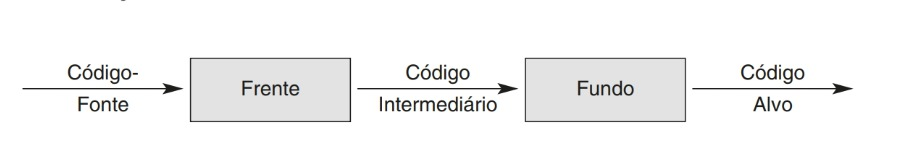
\includegraphics[width=0.7\textwidth]{EsquemaDeCompilador.png}
  \caption{Esquema do funcionamento de um compilador.}
  \label{fig:esquema_compilador}
\end{figure}

O Bloco de Frente ou front-end corresponde ao processo de análise que corresponde a análise léxica, sintática e semântica, já o Fundo ou Back-End gerará através do código intermediário gerado pelo front-end, transformando ele em um código de máquina devidamente otimizado.
Inicialmente esse relatório conterá apenas a parte da análise léxica, mas a medida que o período for passando, outros componentes do compilador serão adicionados. 
O capítulo 2 será referente ao analisador léxico, já o terceiro abordará o sintático, o quarto o semântico e por fim o quinto abordando o desenvolvimento do código alvo que o transforma no código de máquina otimizado.


\section{Analisador Léxico} 

\subsection{Uma breve descrição do que foi solicitado}

Na primeira etapa do trabalho nos foi solicitado inicialmente escolher uma Linguagem de programação simplificada, sendo esse a linguagem C - do livro do Louden, definir um subconjunto de regras de produção e que através das expressões regulares geradas pudéssemos gerar um DFA mínimo sem que houvesse qualquer automatização gerada por qualquer tipo de ferramenta. Além disso, tinhamos que gerar o analisador léxico juntamente com um Scanner para todos os Tokens da BNF escolhida.  
Foi decidido que o scanner seria capaz de ler todas as palavras reservadas e especiais da linguagem proposta pelo Livro do Louden.

\subsection{DFA minimizado e Matriz de Transição}

O Autômato Finito Determinístico minimizado que aceita todas as palavras marcadas e caracteres especiais da linguagem C- é demonstrado abaixo.

\begin{figure}[ht]
    \centering
    \resizebox{\textwidth}{!}{
    \begin{tikzpicture}[
        shorten >=1pt, 
        node distance=2.2cm, 
        on grid, 
        auto, 
        every state/.style={draw=blue!50, very thick, fill=blue!10, minimum size=0.8cm}, 
        initial text= 
    ]

        \node[state, initial] (q_0) {$q_0$};
        
        % WHILE
        \node[state, accepting, above right=of q_0, yshift=4.5cm, xshift=0.5cm] (q_w) {$q_w$};
        \node[state, accepting, right=of q_w] (q_wh) {$q_{wh}$};
        \node[state, accepting, right=of q_wh] (q_whi) {$q_{whi}$};
        \node[state, accepting, right=of q_whi] (q_whil) {$q_{whil}$};
        \node[state, accepting, right=of q_whil] (q_while) {$q_{while}$};

        % IF / INT
        \node[state, accepting, above right=of q_0, yshift=2.8cm, xshift=1.0cm] (q_i) {$q_i$};
        \node[state, accepting, above right=of q_i, yshift=0.4cm, xshift=1cm] (q_if) {$q_{if}$};
        \node[state, accepting, right=of q_i, xshift=0.5cm] (q_in) {$q_{in}$};
        \node[state, accepting, right=of q_in] (q_int) {$q_{int}$};

        % RETURN / VOID / ELSE
        \node[state, accepting, right=of q_0, yshift=3.8cm, xshift=0.5cm] (q_r) {$q_r$};
        \node[state, accepting, right=of q_r] (q_re) {$q_{re}$};
        \node[state, accepting, right=of q_re] (q_ret) {$q_{ret}$};
        \node[state, accepting, right=of q_ret] (q_retu) {$q_{retu}$};
        \node[state, accepting, right=of q_retu] (q_retur) {$q_{retur}$};
        \node[state, accepting, right=of q_retur] (q_return) {$q_{return}$};

        \node[state, accepting, right=of q_0, yshift=2.4cm, xshift=0.5cm] (q_v) {$q_v$};
        \node[state, accepting, right=of q_v] (q_vo) {$q_{vo}$};
        \node[state, accepting, right=of q_vo] (q_voi) {$q_{voi}$};
        \node[state, accepting, right=of q_voi] (q_void) {$q_{void}$};

        \node[state, accepting, right=of q_0, yshift=1.2cm, xshift=0.5cm] (q_e) {$q_e$};
        \node[state, accepting, right=of q_e] (q_el) {$q_{el}$};
        \node[state, accepting, right=of q_el] (q_els) {$q_{els}$};
        \node[state, accepting, right=of q_els] (q_else) {$q_{else}$};

        % QID / QNUM
        \node[state, accepting, right=of q_0, yshift=0.1cm, xshift=3.5cm] (q_id) {$q_{id}$};
        \node[state, accepting, right=of q_0, yshift=-0.8cm, xshift=3.5cm] (q_num) {$q_{num}$};

        % ==========================================
        % 2. ESTADOS DO CADERNO (OPERADORES E DELIMITADORES)
        % ==========================================
        
        % Aritméticos simples (+, -, *)
        \node[state, accepting, below right=of q_0, yshift=0.8cm, xshift=0.2cm] (q_26) {$q_{26}$};
        \node[state, accepting, below right=of q_0, yshift=0.1cm, xshift=0.2cm] (q_27) {$q_{27}$};
        \node[state, accepting, below right=of q_0, yshift=-0.6cm, xshift=0.2cm] (q_28) {$q_{28}$};
        
        % Comentário de Bloco /* ... */
        \node[state, accepting, below right=of q_0, yshift=-1.3cm, xshift=0.2cm] (q_29) {$q_{29}$};
        \node[state, right=of q_29, xshift=1cm] (q_30) {$q_{30}$};
        \node[state, right=of q_30, xshift=1cm] (q_31) {$q_{31}$};
        \node[state, accepting, right=of q_31, xshift=1cm] (q_32) {$q_{32}$};

        % Relacionais Compostos (=, !, >, <)
        \node[state, accepting, below right=of q_0, yshift=-2.2cm, xshift=0.5cm] (q_33) {$q_{33}$};
        \node[state, accepting, right=of q_33] (q_34) {$q_{34}$};

        \node[state, below right=of q_0, yshift=-3.0cm, xshift=0.5cm] (q_35) {$q_{35}$};
        \node[state, accepting, right=of q_35] (q_36) {$q_{36}$};

        \node[state, accepting, below right=of q_0, yshift=-3.8cm, xshift=0.5cm] (q_37) {$q_{37}$};
        \node[state, accepting, right=of q_37] (q_38) {$q_{38}$};

        \node[state, accepting, below right=of q_0, yshift=-4.6cm, xshift=0.5cm] (q_39) {$q_{39}$};
        \node[state, accepting, right=of q_39] (q_40) {$q_{40}$};

        % Delimitadores Unitários Isolados (Coluna vertical abaixo de q0)
        \node[state, accepting, below=of q_0, yshift=-1.5cm, xshift=-1.5cm] (q_41) {$q_{41}$};
        \node[state, accepting, below=of q_41, yshift=1.4cm] (q_42) {$q_{42}$};
        \node[state, accepting, below=of q_42, yshift=1.4cm] (q_43) {$q_{43}$};
        \node[state, accepting, below=of q_43, yshift=1.4cm] (q_44) {$q_{44}$};
        \node[state, accepting, below=of q_44, yshift=1.4cm] (q_45) {$q_{45}$};
        \node[state, accepting, below=of q_45, yshift=1.4cm] (q_46) {$q_{46}$};
        \node[state, accepting, below=of q_46, yshift=1.4cm] (q_47) {$q_{47}$};
        \node[state, accepting, below=of q_47, yshift=1.4cm] (q_48) {$q_{48}$};

        % ==========================================
        % 3. TRANSIÇÕES (SETAS)
        % ==========================================
        \path[->, >=stealth, thick]
            % Palavras-chave anteriores
            (q_0)    edge [bend left=30] node {[w]} (q_w)
            (q_w)    edge node {[h]} (q_wh)
            (q_wh)   edge node {[i]} (q_whi)
            (q_whi)  edge node {[l]} (q_whil)
            (q_whil) edge node {[e]} (q_while)
            (q_0)    edge [bend left=20] node {[i]} (q_i)
            (q_i)    edge [bend left=15] node {[f]} (q_if)
            (q_i)    edge node {[n]} (q_in)
            (q_in)   edge node {[t]} (q_int)
            (q_0)    edge [bend left=25] node {[r]} (q_r)
            (q_r)    edge node {[e]} (q_re)
            (q_re)   edge node {[t]} (q_ret)
            (q_ret)  edge node {[u]} (q_retu)
            (q_retu) edge node {[r]} (q_retur)
            (q_retur) edge node {[n]} (q_return)
            (q_0)    edge [bend left=15] node {[v]} (q_v)
            (q_v)    edge node {[o]} (q_vo)
            (q_vo)   edge node {[i]} (q_voi)
            (q_voi)  edge node {[d]} (q_void)
            (q_0)    edge [bend left=5] node {[e]} (q_e)
            (q_e)    edge node {[l]} (q_el)
            (q_el)   edge node {[s]} (q_els)
            (q_els)  edge node {[e]} (q_else)
            (q_0)    edge [bend right=5] node[above left, xshift=-0.2cm] {$[a\text{-}zA\text{-}Z] \setminus \{i, e, w, v, r\}$} (q_id)
            (q_0)    edge [bend right=10] node {[0-9]} (q_num)
            
            % Símbolos e Operadores do Caderno
            (q_0)    edge [bend right=5] node {+} (q_26)
            (q_0)    edge [bend right=8] node {-} (q_27)
            (q_0)    edge [bend right=12] node {*} (q_28)
            
            % Comentário
            (q_0)    edge [bend right=15] node {/} (q_29)
            (q_29)   edge node {*} (q_30)
            (q_30)   edge [loop above] node {$C \setminus \{*\}$} (q_30)
            (q_30)   edge [bend left=15] node {*} (q_31)
            (q_31)   edge [loop above] node {*} (q_31)
            (q_31)   edge [bend left=15] node {$C \setminus \{/, *\}$} (q_30)
            (q_31)   edge node {/} (q_32)

            % Compostos
            (q_0)    edge [bend right=20] node {=} (q_33)
            (q_33)   edge node {=} (q_34)
            (q_0)    edge [bend right=23] node {!} (q_35)
            (q_35)   edge node {=} (q_36)
            (q_0)    edge [bend right=26] node {>} (q_37)
            (q_37)   edge node {=} (q_38)
            (q_0)    edge [bend right=30] node {<} (q_39)
            (q_39)   edge node {=} (q_40)

            % Delimitadores
            (q_0)    edge [bend right=45] node {;} (q_41)
            (q_0)    edge [bend right=50] node {,} (q_42)
            (q_0)    edge [bend right=55] node {(} (q_43)
            (q_0)    edge [bend right=60] node {)} (q_44)
            (q_0)    edge [bend right=65] node {[} (q_45)
            (q_0)    edge [bend right=70] node {]} (q_46)
            (q_0)    edge [bend right=75] node {\{} (q_47)
            (q_0)    edge [bend right=80] node {\}} (q_48);

    \end{tikzpicture}
    }
    \caption{DFA minimizado final unificado com palavras-chave, operadores e símbolos especiais.}
\end{figure}


\begin{landscape}
\begin{table}[htbp]
\centering
\caption{Matriz de Transição do AFD (simplificada por classes de equivalência de caracteres).}
\label{tab:matriz_transicao}
\setlength{\tabcolsep}{2.5pt} 
\scriptsize

\begin{tabular}{|c|c|ccccc|ccccccccc|c|c|c|c|c|c|}
\hline
\textbf{Estado} & \textbf{$L_{outra}$} & \textbf{e} & \textbf{i} & \textbf{r} & \textbf{v} & \textbf{w} & \textbf{d} & \textbf{f} & \textbf{h} & \textbf{l} & \textbf{n} & \textbf{o} & \textbf{s} & \textbf{t} & \textbf{u} & \textbf{[0-9]} & \textbf{=} & \textbf{/} & \textbf{*} & \textbf{!/$>$/$<$} & \textbf{Outros} \\
\hline
$q_0$ & $q_{ID}$ & $q_e$ & $q_i$ & $q_r$ & $q_v$ & $q_w$ & $q_{ID}$ & $q_{ID}$ & $q_{ID}$ & $q_{ID}$ & $q_{ID}$ & $q_{ID}$ & $q_{ID}$ & $q_{ID}$ & $q_{ID}$ & $q_{num}$ & $q_{ASSIGN}$ & $q_{/}$ & $q_*$ & $q_{op}$ & $q_{simb}$ \\
$q_i$ & $q_{ID}$ & $q_{ID}$ & $q_{ID}$ & $q_{ID}$ & $q_{ID}$ & $q_{ID}$ & $q_{ID}$ & $q_{if}$ & $q_{ID}$ & $q_{ID}$ & $q_{in}$ & $q_{ID}$ & $q_{ID}$ & $q_{ID}$ & $q_{ID}$ & $q_{erro}$ & $q_{erro}$ & $q_{erro}$ & $q_{erro}$ & $q_{erro}$ & $q_{erro}$ \\
$q_{if}$ & $q_{ID}$ & $q_{ID}$ & $q_{ID}$ & $q_{ID}$ & $q_{ID}$ & $q_{ID}$ & $q_{ID}$ & $q_{ID}$ & $q_{ID}$ & $q_{ID}$ & $q_{ID}$ & $q_{ID}$ & $q_{ID}$ & $q_{ID}$ & $q_{ID}$ & $q_{erro}$ & $q_{erro}$ & $q_{erro}$ & $q_{erro}$ & $q_{erro}$ & $q_{erro}$ \\
$q_{in}$ & $q_{ID}$ & $q_{ID}$ & $q_{ID}$ & $q_{ID}$ & $q_{ID}$ & $q_{ID}$ & $q_{ID}$ & $q_{ID}$ & $q_{ID}$ & $q_{ID}$ & $q_{ID}$ & $q_{ID}$ & $q_{ID}$ & $q_{int}$ & $q_{ID}$ & $q_{erro}$ & $q_{erro}$ & $q_{erro}$ & $q_{erro}$ & $q_{erro}$ & $q_{erro}$ \\
$q_{int}$ & $q_{ID}$ & $q_{ID}$ & $q_{ID}$ & $q_{ID}$ & $q_{ID}$ & $q_{ID}$ & $q_{ID}$ & $q_{ID}$ & $q_{ID}$ & $q_{ID}$ & $q_{ID}$ & $q_{ID}$ & $q_{ID}$ & $q_{ID}$ & $q_{ID}$ & $q_{erro}$ & $q_{erro}$ & $q_{erro}$ & $q_{erro}$ & $q_{erro}$ & $q_{erro}$ \\
$q_w$ & $q_{ID}$ & $q_{ID}$ & $q_{ID}$ & $q_{ID}$ & $q_{ID}$ & $q_{ID}$ & $q_{ID}$ & $q_{ID}$ & $q_{wh}$ & $q_{ID}$ & $q_{ID}$ & $q_{ID}$ & $q_{ID}$ & $q_{ID}$ & $q_{ID}$ & $q_{erro}$ & $q_{erro}$ & $q_{erro}$ & $q_{erro}$ & $q_{erro}$ & $q_{erro}$ \\
$q_{wh}$ & $q_{ID}$ & $q_{ID}$ & $q_{whi}$ & $q_{ID}$ & $q_{ID}$ & $q_{ID}$ & $q_{ID}$ & $q_{ID}$ & $q_{ID}$ & $q_{ID}$ & $q_{ID}$ & $q_{ID}$ & $q_{ID}$ & $q_{ID}$ & $q_{ID}$ & $q_{erro}$ & $q_{erro}$ & $q_{erro}$ & $q_{erro}$ & $q_{erro}$ & $q_{erro}$ \\
$q_{whi}$ & $q_{ID}$ & $q_{ID}$ & $q_{ID}$ & $q_{ID}$ & $q_{ID}$ & $q_{ID}$ & $q_{ID}$ & $q_{ID}$ & $q_{ID}$ & $q_{whil}$ & $q_{ID}$ & $q_{ID}$ & $q_{ID}$ & $q_{ID}$ & $q_{ID}$ & $q_{erro}$ & $q_{erro}$ & $q_{erro}$ & $q_{erro}$ & $q_{erro}$ & $q_{erro}$ \\
$q_{whil}$ & $q_{ID}$ & $q_{while}$ & $q_{ID}$ & $q_{ID}$ & $q_{ID}$ & $q_{ID}$ & $q_{ID}$ & $q_{ID}$ & $q_{ID}$ & $q_{ID}$ & $q_{ID}$ & $q_{ID}$ & $q_{ID}$ & $q_{ID}$ & $q_{ID}$ & $q_{erro}$ & $q_{erro}$ & $q_{erro}$ & $q_{erro}$ & $q_{erro}$ & $q_{erro}$ \\
$q_{while}$ & $q_{ID}$ & $q_{ID}$ & $q_{ID}$ & $q_{ID}$ & $q_{ID}$ & $q_{ID}$ & $q_{ID}$ & $q_{ID}$ & $q_{ID}$ & $q_{ID}$ & $q_{ID}$ & $q_{ID}$ & $q_{ID}$ & $q_{ID}$ & $q_{ID}$ & $q_{erro}$ & $q_{erro}$ & $q_{erro}$ & $q_{erro}$ & $q_{erro}$ & $q_{erro}$ \\
$q_e$ & $q_{ID}$ & $q_{ID}$ & $q_{ID}$ & $q_{ID}$ & $q_{ID}$ & $q_{ID}$ & $q_{ID}$ & $q_{ID}$ & $q_{ID}$ & $q_{el}$ & $q_{ID}$ & $q_{ID}$ & $q_{ID}$ & $q_{ID}$ & $q_{ID}$ & $q_{erro}$ & $q_{erro}$ & $q_{erro}$ & $q_{erro}$ & $q_{erro}$ & $q_{erro}$ \\
$q_{el}$ & $q_{ID}$ & $q_{ID}$ & $q_{ID}$ & $q_{ID}$ & $q_{ID}$ & $q_{ID}$ & $q_{ID}$ & $q_{ID}$ & $q_{ID}$ & $q_{ID}$ & $q_{ID}$ & $q_{ID}$ & $q_{els}$ & $q_{ID}$ & $q_{ID}$ & $q_{erro}$ & $q_{erro}$ & $q_{erro}$ & $q_{erro}$ & $q_{erro}$ & $q_{erro}$ \\
$q_{els}$ & $q_{ID}$ & $q_{else}$ & $q_{ID}$ & $q_{ID}$ & $q_{ID}$ & $q_{ID}$ & $q_{ID}$ & $q_{ID}$ & $q_{ID}$ & $q_{ID}$ & $q_{ID}$ & $q_{ID}$ & $q_{ID}$ & $q_{ID}$ & $q_{ID}$ & $q_{erro}$ & $q_{erro}$ & $q_{erro}$ & $q_{erro}$ & $q_{erro}$ & $q_{erro}$ \\
$q_{else}$ & $q_{ID}$ & $q_{ID}$ & $q_{ID}$ & $q_{ID}$ & $q_{ID}$ & $q_{ID}$ & $q_{ID}$ & $q_{ID}$ & $q_{ID}$ & $q_{ID}$ & $q_{ID}$ & $q_{ID}$ & $q_{ID}$ & $q_{ID}$ & $q_{ID}$ & $q_{erro}$ & $q_{erro}$ & $q_{erro}$ & $q_{erro}$ & $q_{erro}$ & $q_{erro}$ \\
$q_v$ & $q_{ID}$ & $q_{ID}$ & $q_{ID}$ & $q_{ID}$ & $q_{ID}$ & $q_{ID}$ & $q_{ID}$ & $q_{ID}$ & $q_{ID}$ & $q_{ID}$ & $q_{ID}$ & $q_{vo}$ & $q_{ID}$ & $q_{ID}$ & $q_{ID}$ & $q_{erro}$ & $q_{erro}$ & $q_{erro}$ & $q_{erro}$ & $q_{erro}$ & $q_{erro}$ \\
$q_{vo}$ & $q_{ID}$ & $q_{ID}$ & $q_{voi}$ & $q_{ID}$ & $q_{ID}$ & $q_{ID}$ & $q_{ID}$ & $q_{ID}$ & $q_{ID}$ & $q_{ID}$ & $q_{ID}$ & $q_{ID}$ & $q_{ID}$ & $q_{ID}$ & $q_{ID}$ & $q_{erro}$ & $q_{erro}$ & $q_{erro}$ & $q_{erro}$ & $q_{erro}$ & $q_{erro}$ \\
$q_{voi}$ & $q_{ID}$ & $q_{ID}$ & $q_{ID}$ & $q_{ID}$ & $q_{ID}$ & $q_{ID}$ & $q_{void}$ & $q_{ID}$ & $q_{ID}$ & $q_{ID}$ & $q_{ID}$ & $q_{ID}$ & $q_{ID}$ & $q_{ID}$ & $q_{ID}$ & $q_{erro}$ & $q_{erro}$ & $q_{erro}$ & $q_{erro}$ & $q_{erro}$ & $q_{erro}$ \\
$q_{void}$ & $q_{ID}$ & $q_{ID}$ & $q_{ID}$ & $q_{ID}$ & $q_{ID}$ & $q_{ID}$ & $q_{ID}$ & $q_{ID}$ & $q_{ID}$ & $q_{ID}$ & $q_{ID}$ & $q_{ID}$ & $q_{ID}$ & $q_{ID}$ & $q_{ID}$ & $q_{erro}$ & $q_{erro}$ & $q_{erro}$ & $q_{erro}$ & $q_{erro}$ & $q_{erro}$ \\
$q_r$ & $q_{ID}$ & $q_{re}$ & $q_{ID}$ & $q_{ID}$ & $q_{ID}$ & $q_{ID}$ & $q_{ID}$ & $q_{ID}$ & $q_{ID}$ & $q_{ID}$ & $q_{ID}$ & $q_{ID}$ & $q_{ID}$ & $q_{ID}$ & $q_{ID}$ & $q_{erro}$ & $q_{erro}$ & $q_{erro}$ & $q_{erro}$ & $q_{erro}$ & $q_{erro}$ \\
$q_{re}$ & $q_{ID}$ & $q_{ID}$ & $q_{ID}$ & $q_{ID}$ & $q_{ID}$ & $q_{ID}$ & $q_{ID}$ & $q_{ID}$ & $q_{ID}$ & $q_{ID}$ & $q_{ID}$ & $q_{ID}$ & $q_{ID}$ & $q_{ret}$ & $q_{ID}$ & $q_{erro}$ & $q_{erro}$ & $q_{erro}$ & $q_{erro}$ & $q_{erro}$ & $q_{erro}$ \\
$q_{ret}$ & $q_{ID}$ & $q_{ID}$ & $q_{ID}$ & $q_{ID}$ & $q_{ID}$ & $q_{ID}$ & $q_{ID}$ & $q_{ID}$ & $q_{ID}$ & $q_{ID}$ & $q_{ID}$ & $q_{ID}$ & $q_{ID}$ & $q_{ID}$ & $q_{retu}$ & $q_{erro}$ & $q_{erro}$ & $q_{erro}$ & $q_{erro}$ & $q_{erro}$ & $q_{erro}$ \\
$q_{retu}$ & $q_{ID}$ & $q_{ID}$ & $q_{ID}$ & $q_{retur}$ & $q_{ID}$ & $q_{ID}$ & $q_{ID}$ & $q_{ID}$ & $q_{ID}$ & $q_{ID}$ & $q_{ID}$ & $q_{ID}$ & $q_{ID}$ & $q_{ID}$ & $q_{ID}$ & $q_{erro}$ & $q_{erro}$ & $q_{erro}$ & $q_{erro}$ & $q_{erro}$ & $q_{erro}$ \\
$q_{retur}$ & $q_{ID}$ & $q_{ID}$ & $q_{ID}$ & $q_{ID}$ & $q_{ID}$ & $q_{ID}$ & $q_{ID}$ & $q_{ID}$ & $q_{ID}$ & $q_{ID}$ & $q_{return}$ & $q_{ID}$ & $q_{ID}$ & $q_{ID}$ & $q_{ID}$ & $q_{erro}$ & $q_{erro}$ & $q_{erro}$ & $q_{erro}$ & $q_{erro}$ & $q_{erro}$ \\
$q_{return}$ & $q_{ID}$ & $q_{ID}$ & $q_{ID}$ & $q_{ID}$ & $q_{ID}$ & $q_{ID}$ & $q_{ID}$ & $q_{ID}$ & $q_{ID}$ & $q_{ID}$ & $q_{ID}$ & $q_{ID}$ & $q_{ID}$ & $q_{ID}$ & $q_{ID}$ & $q_{erro}$ & $q_{erro}$ & $q_{erro}$ & $q_{erro}$ & $q_{erro}$ & $q_{erro}$ \\
$q_{ID}$ & $q_{ID}$ & $q_{ID}$ & $q_{ID}$ & $q_{ID}$ & $q_{ID}$ & $q_{ID}$ & $q_{ID}$ & $q_{ID}$ & $q_{ID}$ & $q_{ID}$ & $q_{ID}$ & $q_{ID}$ & $q_{ID}$ & $q_{ID}$ & $q_{ID}$ & $q_{erro}$ & $q_{erro}$ & $q_{erro}$ & $q_{erro}$ & $q_{erro}$ & $q_{erro}$ \\
$q_{num}$ & $q_{erro}$ & $q_{erro}$ & $q_{erro}$ & $q_{erro}$ & $q_{erro}$ & $q_{erro}$ & $q_{erro}$ & $q_{erro}$ & $q_{erro}$ & $q_{erro}$ & $q_{erro}$ & $q_{erro}$ & $q_{erro}$ & $q_{erro}$ & $q_{erro}$ & $q_{num}$ & $q_{erro}$ & $q_{erro}$ & $q_{erro}$ & $q_{erro}$ & $q_{erro}$ \\
$q_{/}$ & $q_{erro}$ & $q_{erro}$ & $q_{erro}$ & $q_{erro}$ & $q_{erro}$ & $q_{erro}$ & $q_{erro}$ & $q_{erro}$ & $q_{erro}$ & $q_{erro}$ & $q_{erro}$ & $q_{erro}$ & $q_{erro}$ & $q_{erro}$ & $q_{erro}$ & $q_{erro}$ & $q_{erro}$ & $q_{erro}$ & $q_{/*}$ & $q_{erro}$ & $q_{erro}$ \\
$q_{/*}$ & $q_{/*}$ & $q_{/*}$ & $q_{/*}$ & $q_{/*}$ & $q_{/*}$ & $q_{/*}$ & $q_{/*}$ & $q_{/*}$ & $q_{/*}$ & $q_{/*}$ & $q_{/*}$ & $q_{/*}$ & $q_{/*}$ & $q_{/*}$ & $q_{/*}$ & $q_{/*}$ & $q_{/*}$ & $q_{/*}$ & $q_{/**}$ & $q_{/*}$ & $q_{/*}$ \\
$q_{/**}$ & $q_{/*}$ & $q_{/*}$ & $q_{/*}$ & $q_{/*}$ & $q_{/*}$ & $q_{/*}$ & $q_{/*}$ & $q_{/*}$ & $q_{/*}$ & $q_{/*}$ & $q_{/*}$ & $q_{/*}$ & $q_{/*}$ & $q_{/*}$ & $q_{/*}$ & $q_{/*}$ & $q_{/*}$ & $q_{COMMENT}$ & $q_{/**}$ & $q_{/*}$ & $q_{/*}$ \\
$q_{ASSIGN}$ & $q_{erro}$ & $q_{erro}$ & $q_{erro}$ & $q_{erro}$ & $q_{erro}$ & $q_{erro}$ & $q_{erro}$ & $q_{erro}$ & $q_{erro}$ & $q_{erro}$ & $q_{erro}$ & $q_{erro}$ & $q_{erro}$ & $q_{erro}$ & $q_{erro}$ & $q_{erro}$ & $q_{EQUAL}$ & $q_{erro}$ & $q_{erro}$ & $q_{erro}$ & $q_{erro}$ \\
$q_{!}$ & $q_{erro}$ & $q_{erro}$ & $q_{erro}$ & $q_{erro}$ & $q_{erro}$ & $q_{erro}$ & $q_{erro}$ & $q_{erro}$ & $q_{erro}$ & $q_{erro}$ & $q_{erro}$ & $q_{erro}$ & $q_{erro}$ & $q_{erro}$ & $q_{erro}$ & $q_{erro}$ & $q_{NOTEQUAL}$ & $q_{erro}$ & $q_{erro}$ & $q_{erro}$ & $q_{erro}$ \\
$q_>$ & $q_{erro}$ & $q_{erro}$ & $q_{erro}$ & $q_{erro}$ & $q_{erro}$ & $q_{erro}$ & $q_{erro}$ & $q_{erro}$ & $q_{erro}$ & $q_{erro}$ & $q_{erro}$ & $q_{erro}$ & $q_{erro}$ & $q_{erro}$ & $q_{erro}$ & $q_{erro}$ & $q_{MAIORIGUAL}$ & $q_{erro}$ & $q_{erro}$ & $q_{erro}$ & $q_{erro}$ \\
\hline
\end{tabular}
\end{table}
\end{landscape}

A Tabela \ref{tab:matriz_transicao} apresenta a matriz de transição do DFA. 
Para fins de legibilidade e síntese da representação, os caracteres de entrada foram agrupados nas seguintes classes de equivalência: \newline
$L_{outras}$: 
Conjunto de letras maiúsculas e minúsculas $[A\text{-}Z, a\text{-}z]$ que não iniciam nem compõem caminhos de palavras reservadas (ex: $a, b, c, g, j, k, m, p, q, x, y, z$).\newline
$[0\text{-}9]$: 
Todos os dígitos numéricos de 0 a 9.\newline
$! / > / <$: Operadores relacionais simples que podem compor operadores duplos com $=$ (gerando $q_{NOTEQUAL}$, $q_{MAIORIGUAL}$, etc.).\newline
Outros: Delimitadores e operadores de caractere único ($+, -, ,, ;, (, ), [, ], \{, \}$) cujas transições a partir de $q_0$ levam diretamente ao seu estado final individual e geram erro em outros estados.

\subsection{O Scanner}

\subsection{FLEX gerado da BNF}

Uma das atividades solicitadas foi a geração do analisador léxico com FLEX, contendo todas as regras da BNF. 
O propósito principal para a geração do scanner em FLEX é para conferir se as saídas geradas pelo nosso scanner estão corretas. 
Ele está dividido em 3 partes. Definição, regras e Código. A primeira coisa feita foi a geração de um buffer com capacidade de 4096 bytes, 
que serve de limite para a escrita dos tokens, a variável linha atual que é um simples contador, muito útil para dar relatórios, 
indicando em qual linha ocorreu os erros léxicos. Além disso todas as regras envolvendo as palavras reservadas, identificadores, caracteres especiais e números estão indicados da linha 13 até a 68 de acordo com as suas regras. 
Uma das grandes dificuldades no uso do FLEX pra gerar a BNF foi se acostumar com a sintaxe dos comandos e das regras em si inicialmente. 
Após isso a maior dificuldade foi na geração do token de comentário, sendo necessário um conjunto de diversas regras que relacionam-se entre si para ser gerado. 
Uma dificuldade secundária também foi o costume do uso do uso dos comandos pelo terminal, sendo que inicialmente a criação do FLEX foi feita em um compilador online do FLEX chamado JDoodle para depois ser escrito no nosso código.

\begin{lstlisting}
%{
#include <stdio.h>
#include <string.h>

int linha_atual = 1;


char string_comentario[4096];
%}

%x COMENTARIO

%%
"else"          { printf("(\"%s\", ELSE)\n", yytext); }
"if"            { printf("(\"%s\", IF)\n", yytext); }
"int"           { printf("(\"%s\", INT)\n", yytext); }
"return"        { printf("(\"%s\", RETURN)\n", yytext); }
"void"          { printf("(\"%s\", VOID)\n", yytext); }
"while"         { printf("(\"%s\", WHILE)\n", yytext); }

"+"             { printf("(\"%s\", SOMA)\n", yytext); }
"-"             { printf("(\"%s\", SUB)\n", yytext); }
"*"             { printf("(\"%s\", MULT)\n", yytext); }
"/"             { printf("(\"%s\", DIV)\n", yytext); }

"<="            { printf("(\"%s\", LEQ)\n", yytext); }
"<"             { printf("(\"%s\", LT)\n", yytext); }
">="            { printf("(\"%s\", GEQ)\n", yytext); }
">"             { printf("(\"%s\", GT)\n", yytext); }
"=="            { printf("(\"%s\", EQ)\n", yytext); }
"!="            { printf("(\"%s\", NEQ)\n", yytext); }
"="             { printf("(\"%s\", ASSIGN)\n", yytext); }

";"             { printf("(\"%s\", SEMI)\n", yytext); }
","             { printf("(\"%s\", COMMA)\n", yytext); }
"("             { printf("(\"%s\", LPAREN)\n", yytext); }
")"             { printf("(\"%s\", RPAREN)\n", yytext); }
"["             { printf("(\"%s\", LBRACK)\n", yytext); }
"]"             { printf("(\"%s\", RBRACK)\n", yytext); }
"{"             { printf("(\"%s\", LBRACE)\n", yytext); }
"}"             { printf("(\"%s\", RBRACE)\n", yytext); }

[0-9]+          { printf("(\"%s\", NUM)\n", yytext); }
[a-zA-Z]+       { printf("(\"%s\", ID)\n", yytext); }

"/*"            {
                    /* Inicializa o buffer com o inicio do comentario */
                    strcpy(string_comentario, "/*");
                    BEGIN(COMENTARIO);
                }
<COMENTARIO>"*/" {
                    /* Finaliza o buffer, imprime o token e volta ao normal */
                    strcat(string_comentario, "*/");
                    printf("(\"%s\", COMENTARIO)\n", string_comentario);
                    BEGIN(INITIAL);
                }
<COMENTARIO>\n   {
                    linha_atual++;
                    strcat(string_comentario, yytext);
                }
<COMENTARIO>.    {
                    strcat(string_comentario, yytext);
                }

\n              { linha_atual++; }
[ \t\r]+        { /* ignora espacos vazios */ }
.               { printf("ERRO LEXICO (Linha %d): Caractere inesperado '%s'\n", linha_atual, yytext); }
%%

int yywrap() { return 1; }
int main() { yylex(); return 0; }
\end{lstlisting}

Para averiguar o analisador léxico foram utilizadas 4 instâncias corretas e 4 incorretas. Cada uma com o seu devido grau de complexidade, pois já que todas as palavras reservadas e especiais da linguagem C - foram trazidas, foi considerado por bem, exibir todas elas nos testes. Os testes válidos foram chamados de valido1,valido2,...,valido4 e os inválidos de invalido1, invalido2,...,invalido4. 

\subsection{Resultados obtidos pelo nosso analisador comparado com o scanner gerado pelo FLEX}

Os programas para testes estão sendo exibidos no Appendix A, tanto os testes que não possuem quanto os que possuem erros léxicos estão presentes. Já no anexo B encontra-se os resultados obtidos pelo scanner gerado pelo Flex e o C contendo o nosso Scanner.

\subsection{Conclusão}

Essa pequena história nos mostra que por mais que tentemos escolher o que é considerado o certo, sempre irão ocorrer situações que nos posicionam fora da nossa zona de conforto, colocando a prova nossos valores morais, nos forçando fazer escolhas que são necessárias e que irão definir nosso futuro, nos mostrando que nem sempre vamos poder escolher fazer o certo, mas ter de escolher fazer o necessário, por mais difícil que seja. Várias situações parecidas são postas a nós todos os dias, porém com diferentes magnitudes, o modo como nos portamos diante dessas decisões é o que nos define.


\bibliographystyle{sbc}
\bibliography{sbc-template}

\newpage

\section{Anexos do experimento Envolvendo o Analisador Léxico.}

Agora será exibido abaixo as instâncias usadas para os experimentos.


\begin{appendices}
  % Se o seu documento usa \section (como a classe article)
  \section{Código Fonte dos Programas Validos e Inválidos}
  \label{anexo:codigo}

\begin{figure}[H]
  \centering
  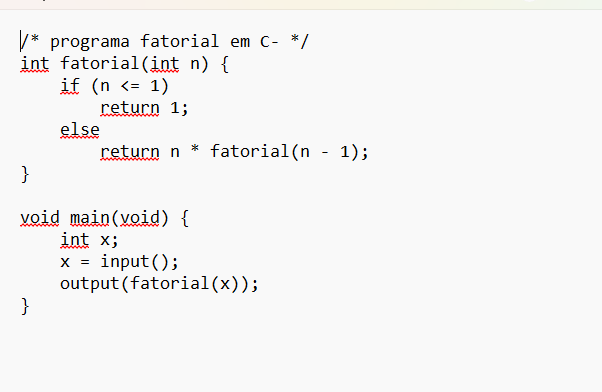
\includegraphics[width=0.7\textwidth]{valido1.png}
  \caption{Programa com resultado válido 1.}
  \label{fig:valido1}
\end{figure}



\begin{figure}[H]
  \centering
  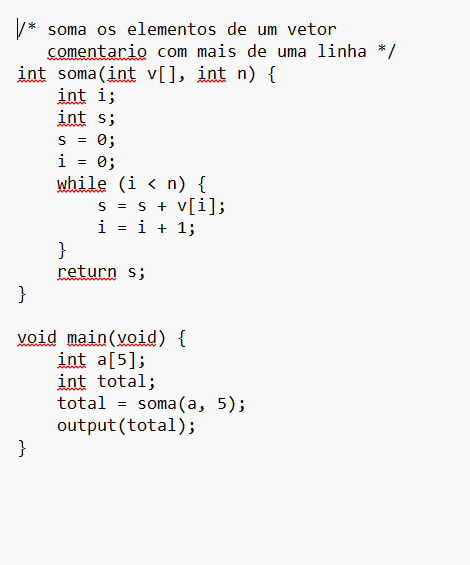
\includegraphics[width=0.7\textwidth]{valido2.png}
  \caption{Programa com resultado válido 2.}
  \label{fig:valido2}
\end{figure}


\begin{figure}[H]
  \centering
  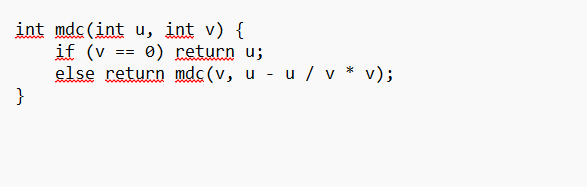
\includegraphics[width=0.7\textwidth]{valido3.png}
  \caption{Programa com resultado válido 3.}
  \label{fig:valido3}
\end{figure}


\begin{figure}[H]
  \centering
  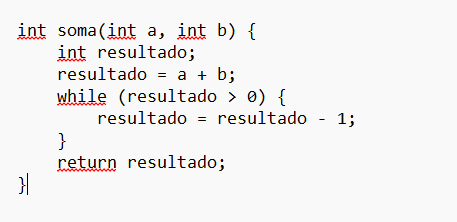
\includegraphics[width=0.7\textwidth]{valido4.png}
  \caption{Programa com resultado válido 4.}
  \label{fig:valido4}
\end{figure}


\begin{figure}[H]
  \centering
  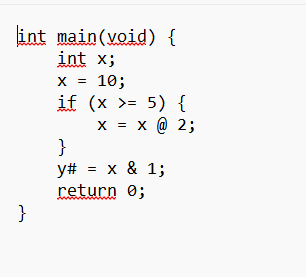
\includegraphics[width=0.7\textwidth]{Invalido1.png}
  \caption{Programa com resultado Invalido 1.}
  \label{fig:invalido1}
\end{figure}


\begin{figure}[H]
  \centering
  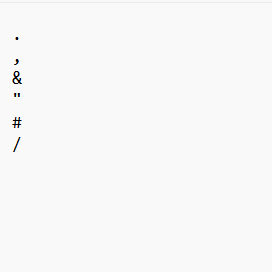
\includegraphics[width=0.7\textwidth]{Invalido2.png}
  \caption{Programa com resultado Invalido 2.}
  \label{fig:invalido2}
\end{figure}


\begin{figure}[H]
  \centering
  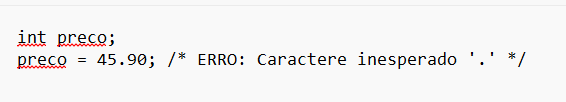
\includegraphics[width=0.7\textwidth]{Invalido3.png}
  \caption{Programa com resultado Invalido 3.}
  \label{fig:invalido3}
\end{figure}



\begin{figure}[H]
  \centering
  
\includegraphics[width=0.7\textwidth]{Invalido4.png}
  \caption{Programa com resultado Invalido 4.}
  \label{fig:invalido4}
\end{figure}




\section{Dados dos Testes Realizados do Scanner flex}
\label{anexo:dados}

\begin{figure}[H]
  \centering
  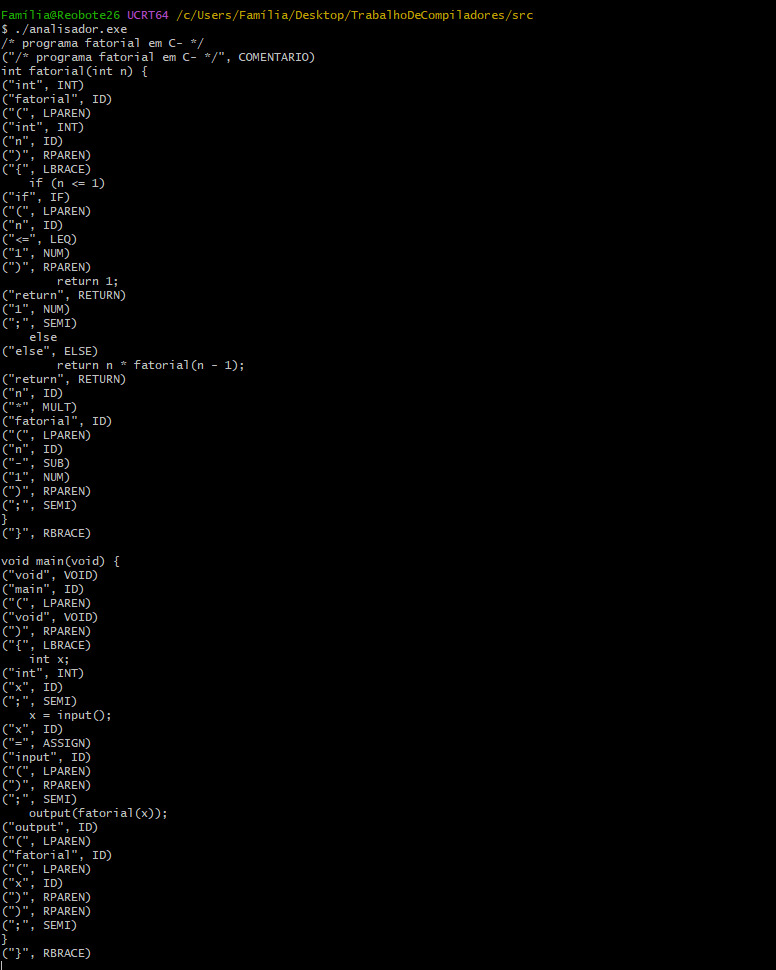
\includegraphics[width=0.7\textwidth]{SolucaoFlexValido1.png}
  \caption{Programa com resultado válido 1.}
  \label{fig:SolucaoFlexValido1}
\end{figure}


\begin{figure}[H]
  \centering
  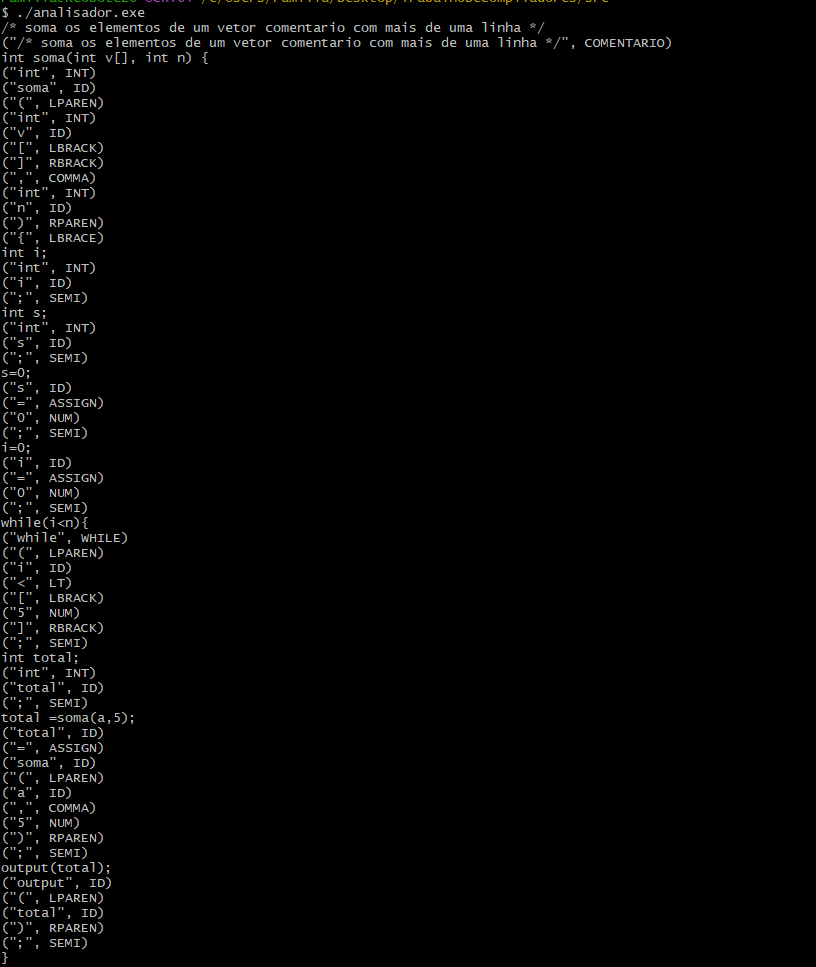
\includegraphics[width=0.7\textwidth]{SolucaoFlexValido2.png}
  \caption{Programa com resultado válido 2.}
  \label{fig:SolucaoFlexValido2}
\end{figure}


\begin{figure}[H]
  \centering
  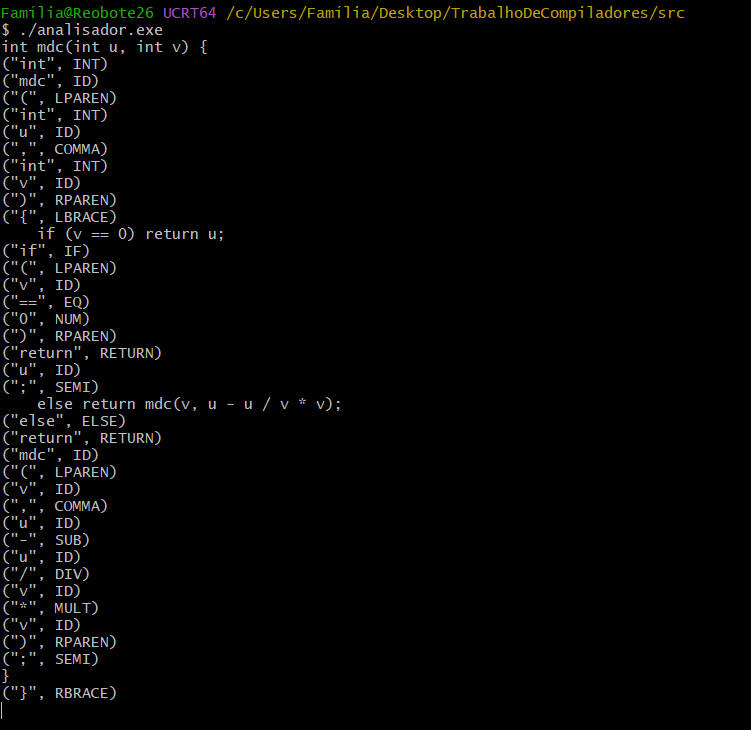
\includegraphics[width=0.7\textwidth]{SolucaoFlexValido3.png}
  \caption{Programa com resultado válido 3.}
  \label{fig:SolucaoFlexValido3}
\end{figure}


\begin{figure}[H]
  \centering
  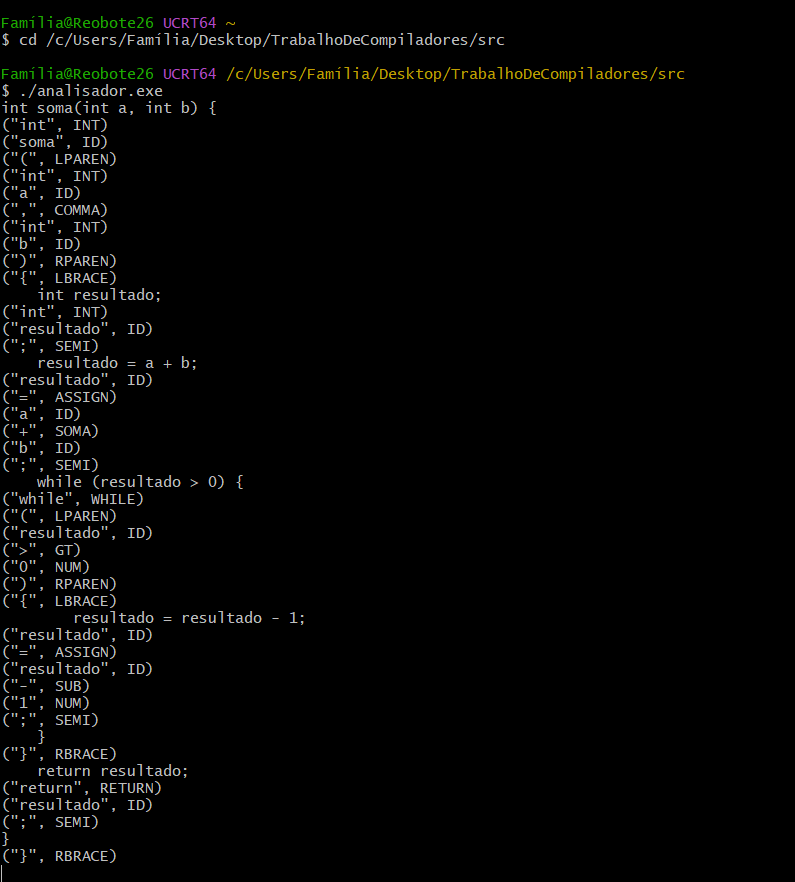
\includegraphics[width=0.7\textwidth]{SolucaoFlexValido4.png}
  \caption{Programa com resultado válido 4.}
  \label{fig:SolucaoFlexValido4}
\end{figure}


\begin{figure}[H]
  \centering
  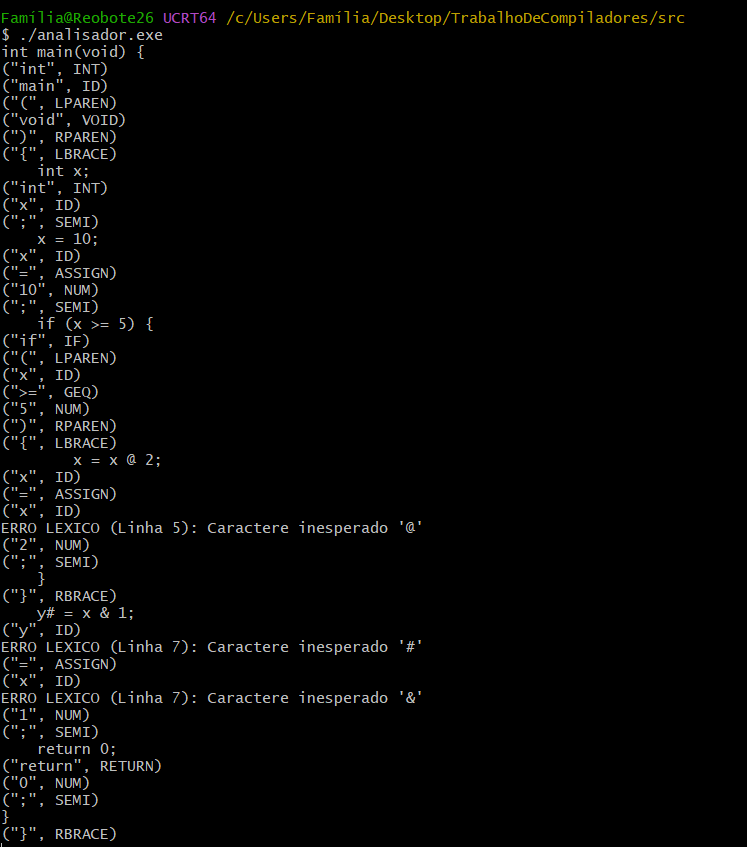
\includegraphics[width=0.7\textwidth]{SolucaoFlexInValido1.png}
  \caption{Programa com resultado Invalido 1.}
  \label{fig:SolucaoFlexInValido1}
\end{figure}

\begin{figure}[H]
  \centering
  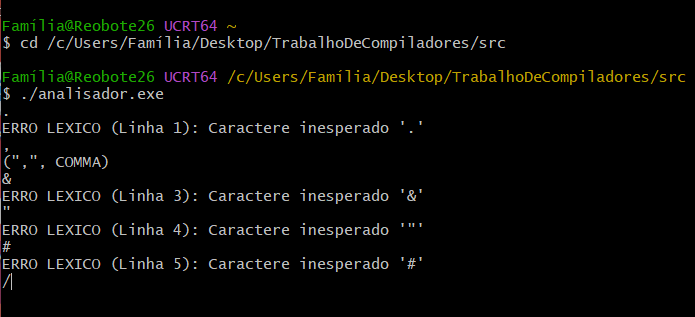
\includegraphics[width=0.7\textwidth]{SolucaoFlexInValido2.png}
  \caption{Programa com resultado Invalido 2.}
  \label{fig:SolucaoFlexInValido2}
\end{figure}

\begin{figure}[H]
  \centering
  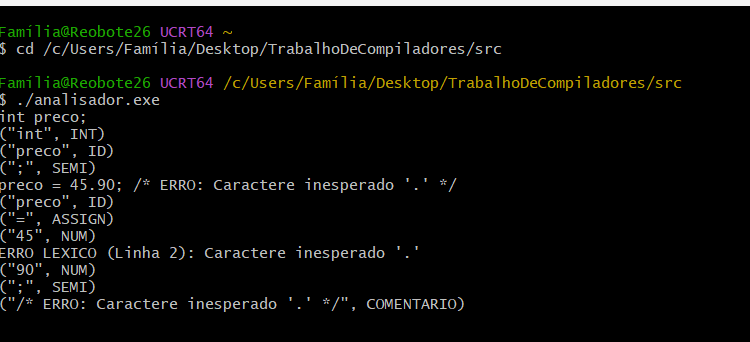
\includegraphics[width=0.7\textwidth]{SolucaoFlexInValido3.png}
  \caption{Programa com resultado Invalido 3.}
  \label{fig:SolucaoFlexInValido3}
\end{figure}


\begin{figure}[H]
  \centering
  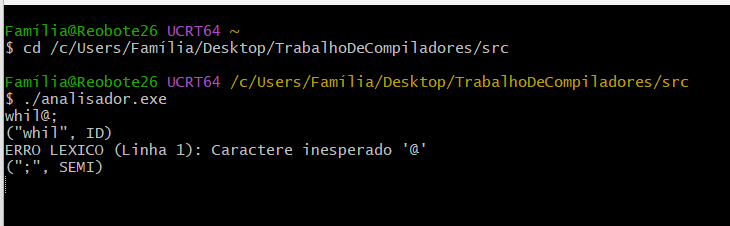
\includegraphics[width=0.7\textwidth]{SolucaoFlexInValido4.png}
  \caption{Programa com resultado Invalido 4.}
  \label{fig:SolucaoFlexInValido4}
\end{figure}

  \section{Dados dos Testes Realizados do Scanner}
  \label{anexo:dados}

  
  \begin{figure}[H]
  \centering
  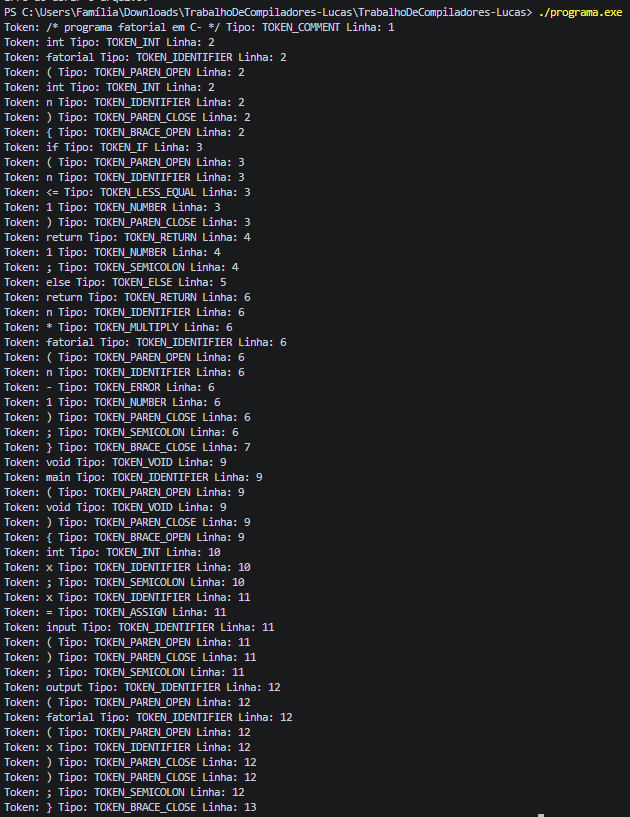
\includegraphics[width=0.7\textwidth]{valido1Scanner.png}
  \caption{Programa com resultado válido 1 do Scanner.}
  \label{fig:valido1Scanner}
\end{figure}


  \begin{figure}[H]
  \centering
  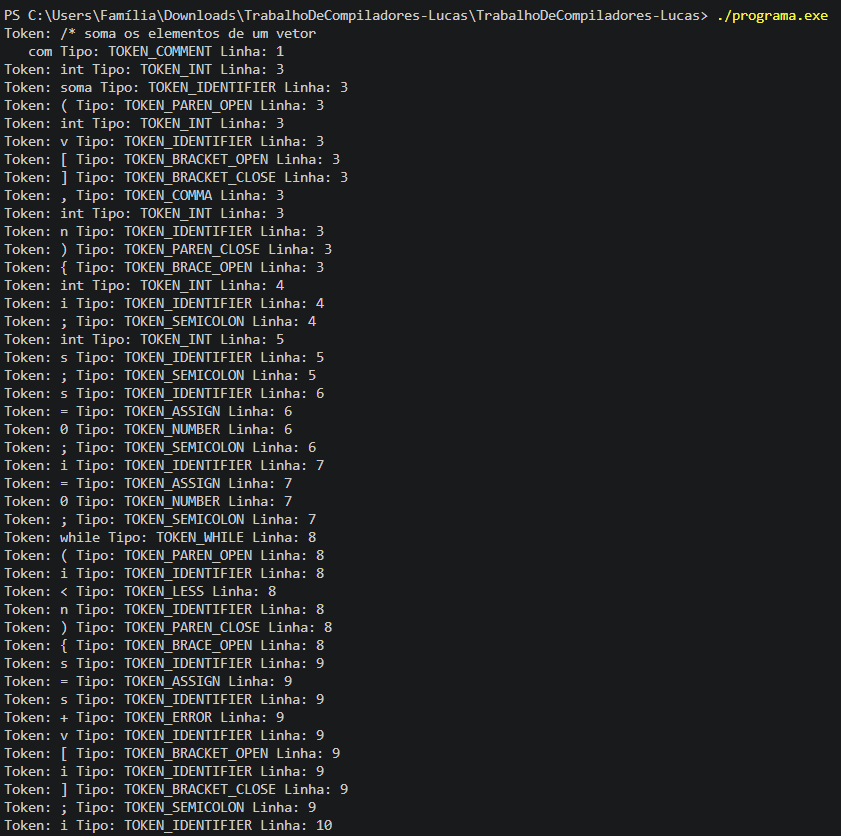
\includegraphics[width=0.7\textwidth]{valido2Scanner.png}
  \caption{Programa com resultado válido 2 do Scanner.}
  \label{fig:valido2Scanner}
\end{figure}


  \begin{figure}[H]
  \centering
  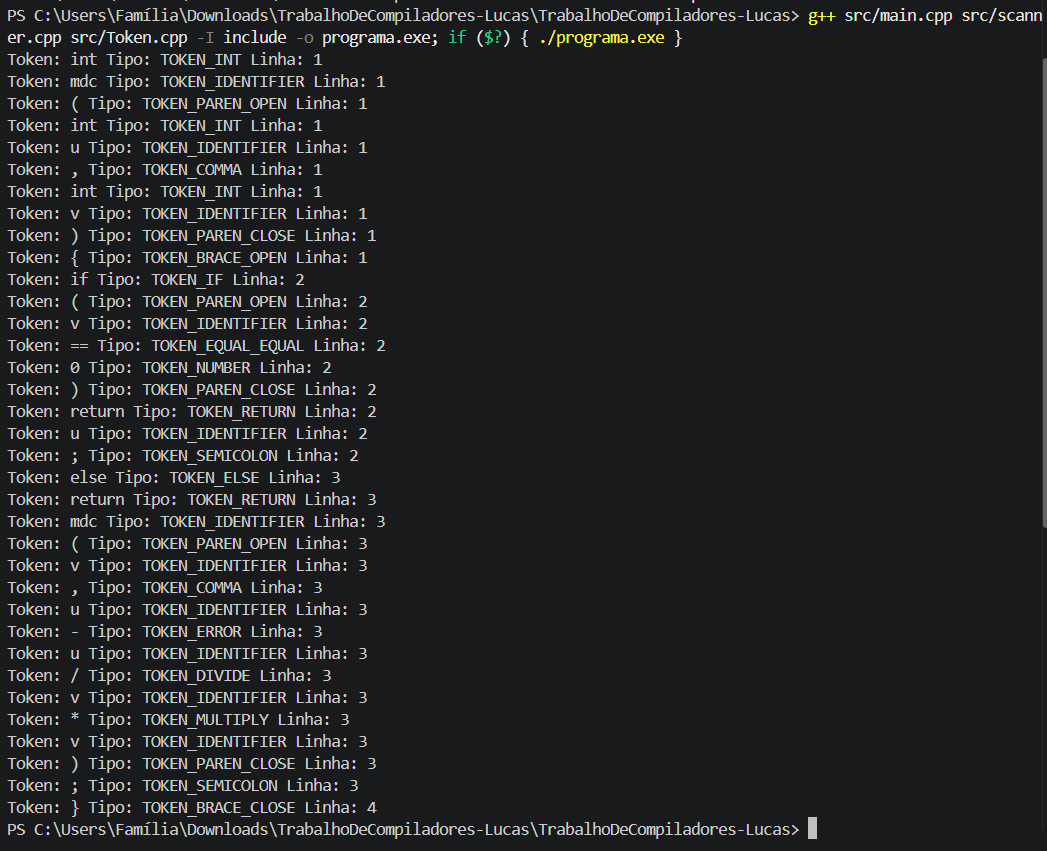
\includegraphics[width=0.7\textwidth]{valido3Scanner.png}
  \caption{Programa com resultado válido 3 do Scanner.}
  \label{fig:valido3Scanner}
\end{figure}

  \begin{figure}[H]
  \centering
  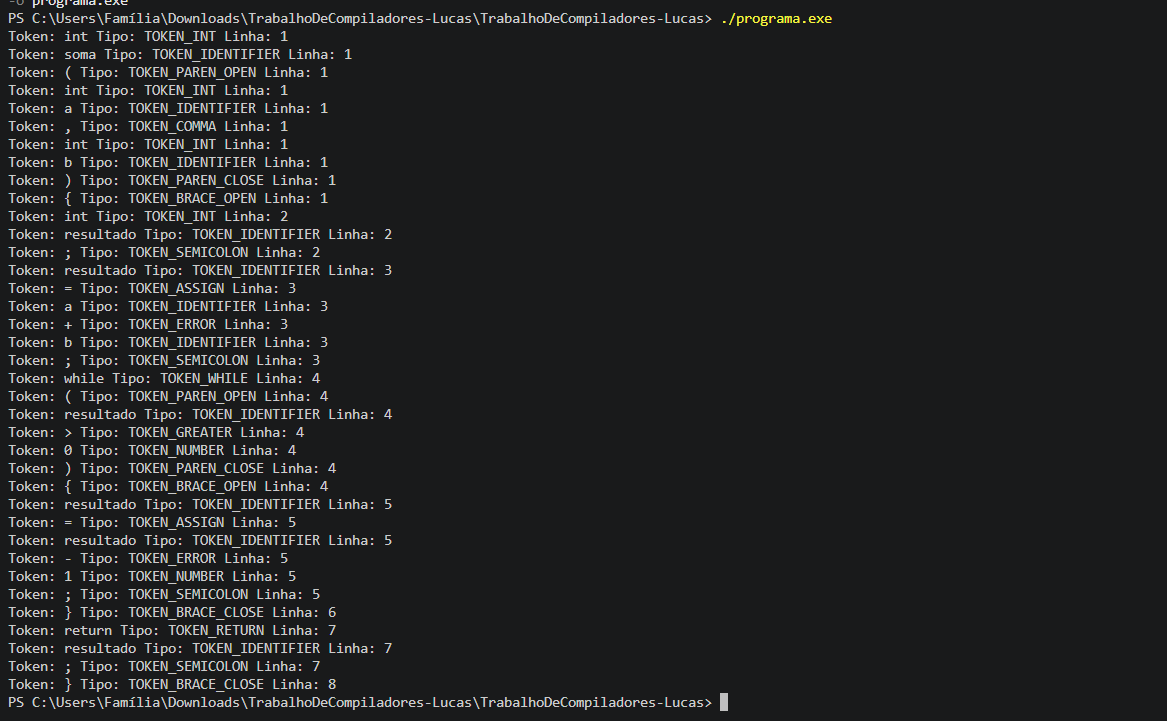
\includegraphics[width=0.7\textwidth]{valido4Scanner.png}
  \caption{Programa com resultado válido 4 do Scanner.}
  \label{fig:valido4Scanner}
\end{figure}

  \begin{figure}[H]
  \centering
  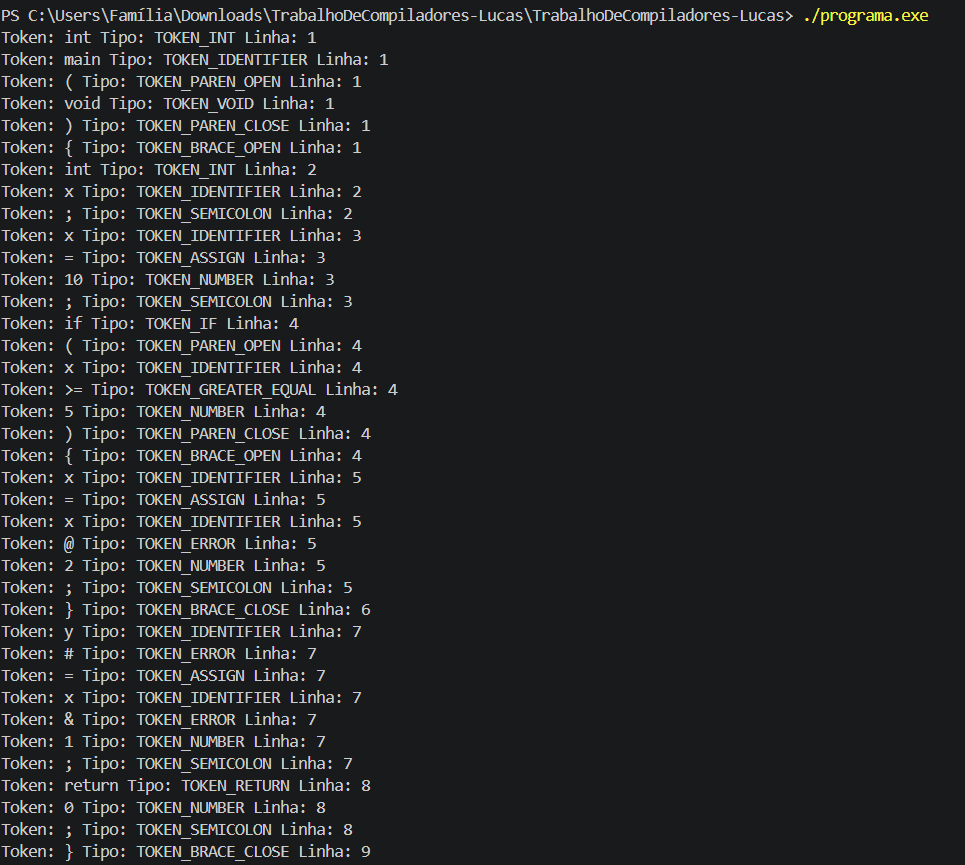
\includegraphics[width=0.7\textwidth]{Invalido1Scanner.png}
  \caption{Programa com resultado inválido 1 do Scanner.}
  \label{fig:Invalido1Scanner}
\end{figure}

  \begin{figure}[H]
  \centering
  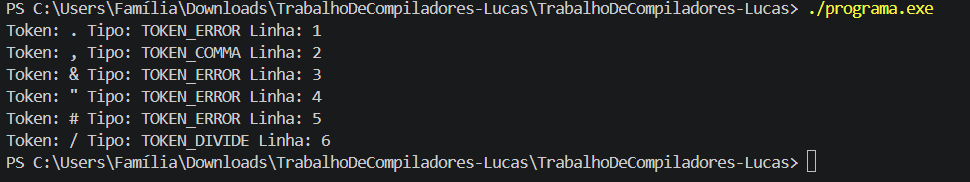
\includegraphics[width=0.7\textwidth]{Invalido2Scanner.png}
  \caption{Programa com resultado inválido 2 do Scanner.}
  \label{fig:Invalido2Scanner}
\end{figure}


  \begin{figure}[H]
  \centering
  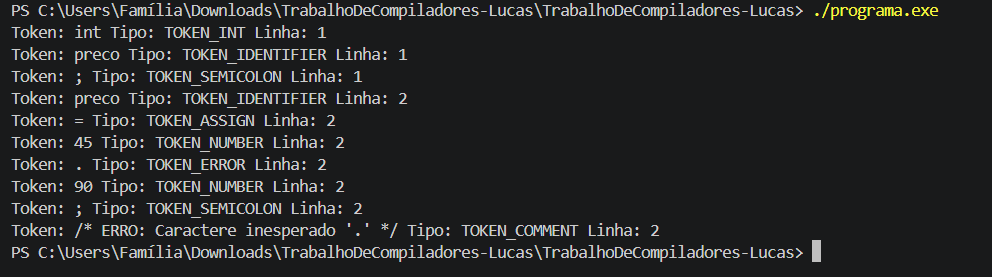
\includegraphics[width=0.7\textwidth]{Invalido3Scanner.png}
  \caption{Programa com resultado inválido 3 do Scanner.}
  \label{fig:Invalido3Scanner}
\end{figure}

  \begin{figure}[H]
  \centering
  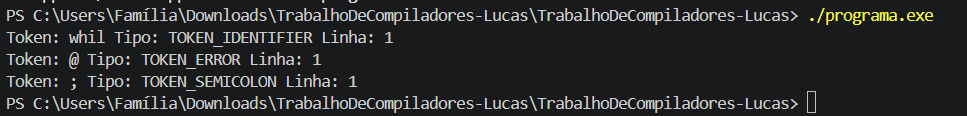
\includegraphics[width=0.7\textwidth]{Invalido4Scanner.png}
  \caption{Programa com resultado inválido 4 do Scanner.}
  \label{fig:Invalido4Scanner}
\end{figure}

\end{appendices}

\end{document}
\end{document}



